\newpage
\section{Methodology and Implementation}
% The system architecture is designed to keep data handling, scenario management, and optimization separate yet 
% interconnected. This structure simplifies extending the model—whether adding more generation types, changing load 
% profiles, or altering cost assumptions. The next section (\S 3.2) will focus on the core components of the 
% mathematical formulation and the integration of financial metrics, such as Net Present Value (NPV) and annuity 
% calculations.

% •	Data Architecture: Clearly separated CSV files for network topology, time-series data, and scenario definitions.
% •	Software Components: A Python-based DCOPF solver with scenario management via main.py, plus optional
% AI-powered summaries.
% •	Flowcharts & Snippets: Recommended visuals and short code excerpts to illustrate data flow (inputs → solver 
% → outputs) and to demonstrate the script’s orchestration logic.
% ensures flexibility in adding or modifying new assets, adapting to different load profiles, and 
% rapidly generating comparative analyses across multiple scenarios.


%---------------------------------------------------------------------------------------
\subsection{System Architecture}
\label{sec:system_architecture}

\subsubsection{Data structure and Input Flow}
\label{sec:input_flow}
The architecture relies on a set of CSV files that define (1) the physical network, (2) the time-series input data, 
and (3) the scenario configurations for analysis. All of these files reside in the \texttt{data/working} directory 
and are ultimately passed to the \texttt{main.py} script, which processes each scenario in turn.

\begin{enumerate}
  \item \textbf{Physical Network Files}: \texttt{branch.csv} and \texttt{bus.csv} \\
  Define the perimeter and physical layout of the power grid in a format inspired by MATPOWER~\cite{matpower2024}. 
  For example, \texttt{branch.csv} provides line impedances and flow limits, while \texttt{bus.csv} specifies bus 
  voltage information, types, and identifiers.
  
  \item \textbf{Time-Series Input Data}: \texttt{master\_gen.csv} and \texttt{master\_load.csv} \\
  One holds the asset-level generation profiles (nuclear, wind, solar, etc.), including capacity 
  limits, per-unit costs, and operational constraints. 
  
  The other one, contains bus-level load profiles, mapped to specific seasonal segments (winter, summer, 
  spring/autumn). These files reflect the availability or demand data relevant to a particular study-case.
  
  \item \textbf{Scenario Configurations}: \texttt{scenarios\_parameters.csv} \\
  Centralizes the definitions of each scenario: which generators or storage units are placed at which buses, along 
  with any load scaling factors (e.g., $\pm20\%$ demand). This dataset dictates how the solver will allocate and 
  dispatch resources in different configurations.
\end{enumerate}

The main driver script, \texttt{multi\_scenario.py}, loads and combines these CSVs to set up each scenario’s 
DCOPF problem. By separating network topologies, time-series inputs, and scenario definitions, the framework 
allows new assets, bus layouts, or experimental conditions to be tested without significant changes to the 
core codebase.

\begin{figure}[H]
    \centering
    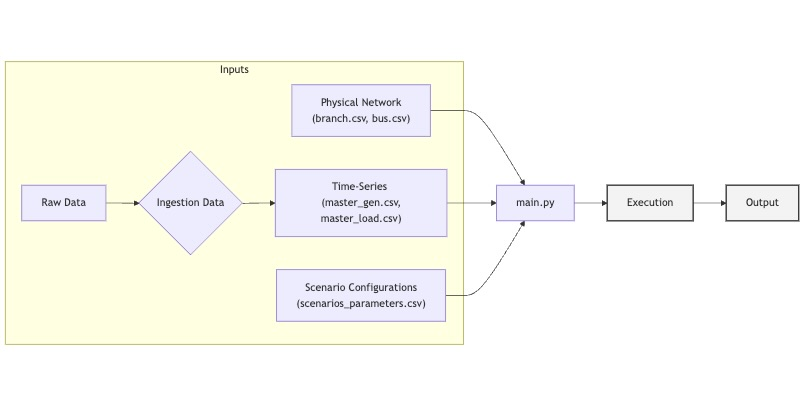
\includegraphics[width=0.75\textwidth]{images/input-flow.jpeg}
    \caption{Overview of the Data Flow into the Optimization Process} \label{fig:input-flow}
\end{figure}

%---
% flowchart LR
%     subgraph Inputs
%       A["Physical Network <br> (branch.csv, bus.csv)"]
%       R["Raw Data"]
%       I{"Ingestion Data"}
%       T["Time-Series <br> (master_gen.csv, master_load.csv)"]
%       C["Scenario Configurations <br> (scenarios_parameters.csv)"]
%     end

%     %% Chain for time-series ingestion
%     R --> I
%     I --> T

%     %% Connect inputs to main processing (main.py)
%     A --> multiScenario[main.py]
%     T --> multiScenario
%     C --> multiScenario

%     %% LP Solver and hidden endpoint
%     multiScenario --> D[Execution]
%     D --> E[Output]

    % %% Define a custom class with a light fill color
    % classDef lightBox fill:#f3f3f3, stroke:#333, stroke-width:2px;

    % %% Apply the custom class to nodes D and E
    % class D,E, lightBox;
%---

\subsubsection{Execution}
\label{sec:execution}
The \texttt{main.py} script serves as the central orchestrator of the optimization workflow.
Its key responsibilities include:

\begin{itemize}
    \item \textbf{Scenario Management}\\
    Loads scenario definitions from \texttt{scenarios\_parameters.csv}, which specify generator placements, storage 
    configurations, and load scaling factors for each test case.
    
    \item \textbf{Data Integration}\\
    Combines network topology data (\texttt{bus.csv}, \texttt{branch.csv}) with time-series inputs 
    (\texttt{master\_gen.csv}, \texttt{master\_load.csv}) to construct complete optimization problems.
    
    \item \textbf{Sensitivity Analysis}\\
    For each base scenario, optionally generates variants with modified load factors (e.g., $\pm20\%$) to test 
    system robustness under different demand conditions.
    
    \item \textbf{Results Collection}\\
    Aggregates solver outputs, calculates key metrics (e.g., capacity factors, annual costs), and stores results 
    in standardized formats for further analysis.
    
    \item \textbf{Investment Analysis}\\
    Interfaces with \texttt{create\_master\_invest.py} to compute financial metrics like NPV and annualized costs 
    across different time horizons.
\end{itemize}

They can be vizualized in the following flowchart:

\begin{figure}[H]
    \centering
    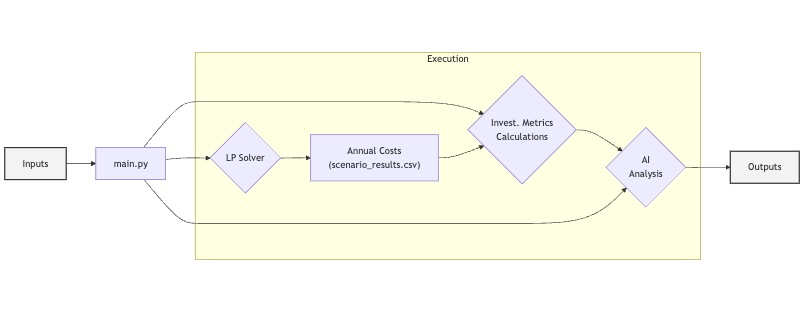
\includegraphics[width=0.75\textwidth]{images/execution-flow.jpeg}
    \caption{Execution and interaction of the main.py script with the other modules}
    \label{fig:execution-flow}
\end{figure}

%---
% flowchart LR

%     subgraph execution [Execution]
%         E
%         G
%         I
%         F
      
%     end

%     D[main.py]
%     %% LP Solver and Annual Costs Calculation
%     D --> E{"LP Solver"}
%     E --> F["Annual Costs <br> (scenario_results.csv)"]

%     %% Investment Analysis
%     D --> G{"Invest. Metrics <br> Calculations"}
%     F --> G
%     G --> K
%     %% Scenario Critic and Reporting
%     D --> I{"AI <br> Analysis"}
%     K --> I
%     I --> J

%     %% Output Files/Structure
%     subgraph Outputs [Outputs]
%         J["Markdown Summary and <br> AI-Generated Reports"]
%         K["Final Scenario Results <br>(scenario_results_with_investment.csv)"]
%         END:::hidden  
%     end
%---

The \texttt{main.py} script also coordinates with auxiliary modules for visualization (\texttt{summary\_plots.py}), 
and documentation updates (\texttt{update\_readme.py}), ensuring up-to-date visualizations and online-documentation.

\subsubsection{Output Flow}
\label{sec:output_flow}
After \texttt{main.py} coordinates the execution of all scenarios through \texttt{dcopf.py}, 
\texttt{create\_master\_invest.py}, and \texttt{summary\_plots.py}, it generates three key outputs:

\begin{itemize}
    \item \textbf{Global Summary Report}\\
    A comprehensive \texttt{summary.md} file that ranks scenarios by annuity value, 
    provides AI-generated insights on overall trends, and includes comparative visualizations across scenarios.

    \item \textbf{Individual Scenario Reports}\\
    For each scenario (e.g., \texttt{scenario\_1\_analysis.md}), it generates a 
    detailed report with: dispatch plots and generation mix charts, financial metrics breakdown, and AI-generated 
    commentary on specific operational patterns.

    \item \textbf{Consolidated Results}\\
    A \texttt{scenario\_results.csv} within \texttt{data/results} containing raw operational
    data (generator dispatch, line flows), investment metrics (NPV, annual costs, annuities), and sensitivity 
    analysis results (if enabled).
\end{itemize}

\noindent
It illustrates the principal output files after interaction with the main.py script and the other modules.

\begin{figure}[H]
    \centering
    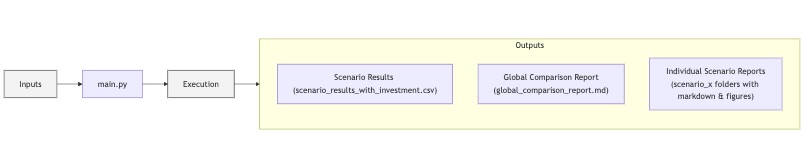
\includegraphics[width=0.75\textwidth]{images/output-flow.jpeg}
    \caption{Output results and reports}
    \label{fig:output-flow}
\end{figure}

%---
% flowchart LR
%     %% LP Solver and Annual Costs Calculation
%     A[Inputs]-->main
%     main[main.py] --> Execution
%     Execution --> Outputs
%     %% Output Files/Structure
%     subgraph Outputs [Outputs]
%       K["Scenario Results <br>(scenario_results_with_investment.csv)"]
%       L["Global Comparison Report<br>(global_comparison_report.md)"]
%       M["Individual Scenario Reports<br>(scenario_x folders with markdown & figures)"]
%     end
%     style Execution fill:#f3f3f3, stroke:#333;
%     style A         fill:#f3f3f3, stroke:#333;
%---

This multi-step workflow ensures all relevant data—raw operational outputs, investment metrics, and optional AI 
insights—remain easily accessible for post-processing or stakeholder review. As a result, users can quickly compare 
scenarios under different configurations, load sensitivities, or asset placements without altering the core solver routines.

% \subsubsection{Illustrative Code Excerpt}
% % Directive: Provide a code snippet from main.py focusing on scenario orchestration.

% The following code snippet from \texttt{main.py} illustrates how scenario parameters are loaded and solved:

% \begin{lstlisting}[
%     language=Python,
%     label={lst:main},
%     caption={Excerpt from main.py illustrating how scenario parameters are loaded and solved},
%     float=htbp
% ]
% # Load scenario definitions
% scenarios_df = pd.read_csv(scenarios_params_file)

% for _, row in scenarios_df.iterrows():
%     scenario_name = row["scenario_name"]
%     gen_positions = parse_positions(row["gen_positions"], data_context['type_to_id'])
%     storage_positions = parse_positions(row["storage_units"], data_context['type_to_id'])
%     base_load_factor = float(row["load_factor"])

%     # Optionally run sensitivity variants: nominal, high (+20%), low (-20%)
%     variants_to_run = [("nominal", base_load_factor)]
%     if run_sensitivity:
%         variants_to_run += [("high", base_load_factor * 1.2),
%                             ("low", base_load_factor * 0.8)]

%     for variant_name, load_factor in variants_to_run:
%         result = run_scenario_variant(
%             scenario_name=scenario_name,
%             gen_positions=gen_positions,
%             storage_positions=storage_positions,
%             load_factor=load_factor,
%             variant=variant_name,
%             data_context=data_context
%         )
%         # Aggregate seasonal results, compute investment metrics, store final
%         ...
        
% \end{lstlisting}

%---------------------------------------------------------------------------------------
\subsection{Core Components}
We detail the four principal building blocks of the project. Their interaction is illustrated in the system 
architecture presented in Section~\ref{sec:system_architecture} by losanges.

\begin{multicols}{2}
\begin{itemize}
  \item LP Optimization Solver (DCOPF)
  \item Data Ingestion \& Preprocessing
\end{itemize}
\columnbreak
\begin{itemize}
  \item Investment Metrics calculation
  \item AI-based reporting
\end{itemize}
\end{multicols}
Each element addresses a distinct requirement, from solving the DC power flow problem to 
generating final scenario reports with optional AI-driven commentary.


\subsubsection{Data Ingestion \& Preprocessing}
\label{sec:data_preprocessing}

\textbf{Data Handling} \\
Data handling follows a three-tiered structure:

\begin{enumerate}
  \item \textbf{\texttt{data/raw}}: Unaltered sources such as annual wind/solar profiles from public 
  databases or raw load curves provided by our supervising professor.

  \item \textbf{\texttt{data/processed}}: Intermediate files that have undergone partial cleaning 
  (e.g., timestamps alignment, filtering outliers). As part of this step, we also perform a 
  \emph{Seasonal and Trend decomposition using Loess (STL)} to identify anomalies in the load profile, following 
  methods described in \cite{predictive_modeling_notes}. The seasonal median week was picked for each season.

  \item \textbf{\texttt{data/working}}: used .csv files directly by the solver and scenario 
  scripts (\texttt{master\_gen.csv}, \texttt{master\_load.csv}). These files are concise, 
  containing only the time-series data and parameters needed for each scenario run.

\end{enumerate}

The STL decomposition applied during the preprocessing step to validate our \emph{typical-week} selection for each 
season (Figure~\ref{fig:stl_load_decomposition}). The data showed a broad U-shaped trend (lower demand in warmer months) and 
strong daily/weekly seasonality. Residuals exhibited higher variance at the start and end of the year, suggesting 
possible holiday or extreme-weather anomalies. Excluding those outlier weeks helped ensure our final “median” week 
captures typical load patterns.

\begin{figure}[H]
    \centering
    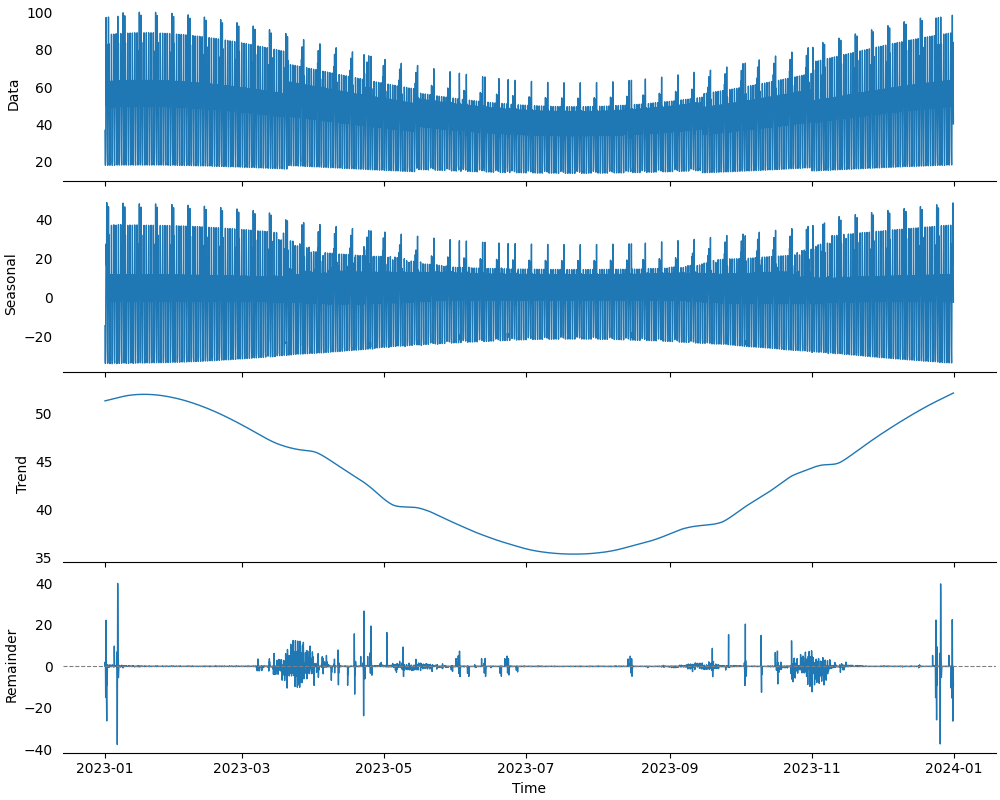
\includegraphics[width=0.6\textwidth]{images/stl-load.png}
    \caption{STL decomposition of the annual load data}
    \label{fig:stl_load_decomposition}
\end{figure}

\textbf{Scripts for Data Preprocessing} \\
Two Python scripts form the backbone of our data preprocessing:

\begin{itemize}
  \item \texttt{create\_master\_gen.py}:
  Consolidates multiple raw generation sources (wind, solar, 
  nuclear, etc.) into a unified time series, selecting a \emph{median week} per season to reduce 
  hours from 8,760 to just $7 \times 24$.

  \item \texttt{create\_master\_load.py}: 
  Builds coherent load profiles for each season, optionally shifting one bus’s demand by a week if needed.
  Buses~5 and~6 serve as the primary load centers in our example network.
\end{itemize}

These scripts output \texttt{master\_gen.csv} and \texttt{master\_load.csv} in \texttt{data/working}.
By scaling each typical week by 13 (winter/summer) or 26 (spring/autumn), the method preserves core 
weekly cycles—consistent with the STL findings—while excluding outlier periods. This provides a 
robust yet computationally efficient basis for annual cost estimation.

\textbf{Network Modeling} \\
A simplified network is defined via \texttt{branch.csv} and \texttt{bus.csv} in \texttt{data/working}. 
Key characteristics of this grid (e.g., line impedances, bus voltage levels) are presented in 
Section~\ref{sec:results}. While our example focuses on a small test system, larger networks 
(e.g., IEEE 30-bus or 118-bus) can be incorporated using the same file structure.


\subsubsection{LP Optimization Solver}
\label{sec:lp_solver}
In this module, the \texttt{dcopf.py} script translates the DC power flow problem and associated operational 
constraints into a linear program (LP). Although the mathematical formulation (objective function and constraints)
has been fully described in Section~\ref{sec:theoretical_background}, we outline here how these elements are 
\emph{implemented} at the code level, focusing on the handling of hourly dispatch and storage dynamics.

\textbf{Time-Step Stacking}\\
For each hour $t$ of the representative dataset (e.g., 24 hours $\times$ 7 days per season), the solver creates:

\begin{itemize}
  \item \textbf{Generation Variables}\\
  It ensures the solver respects asset-level capacity limits in every hour.
  In \texttt{dcopf.py}, each dispatchable asset $g$ is assigned a variable
  \lstinline|GEN[g, t]| that ranges between \lstinline|pmin| and \lstinline|pmax|.
  For each time step $t$, we create:
  \begin{lstlisting}[language=python]
  for g in G:
    for t in T:
        pmin = ...
        pmax = ...
        GEN[g, t] = pulp.LpVariable(
            f"GEN_{g}_{t}_var",
            lowBound=pmin, upBound=pmax)
  \end{lstlisting}

  \item \textbf{Voltage Angles} (Phase Angles) at Each Bus \\
  The DC power flow constraints then enforce line flows based on the angle difference between connected buses.
  A dictionary \lstinline|THETA[i, t]| stores the phase angle at bus $i$ and time $t$:
  \begin{lstlisting}[language=python]
  for i in N:     # set of buses
    for t in T:   # set of time steps
        THETA[i, t] = pulp.LpVariable(
            f"THETA_{i}_{t}_var", lowBound=None, upBound=None)
    \end{lstlisting}
    
  \item \textbf{Line Flow Variables} \\
  For each branch $(i, j)$ in \texttt{branch.csv}, we create \lstinline|FLOW[i, j, t]|,
  constrained by the line's thermal limit (\lstinline|rateA|). The relevant code snippet
  looks like:
  \begin{lstlisting}[language=python]
  for idx, row in branch.iterrows():
    i = int(row['fbus'])
    j = int(row['tbus'])
    limit = row['ratea']
    for t in T:
        FLOW[i, j, t] = pulp.LpVariable(
            f"FLOW_{i}_{j}_{t}_var",
            lowBound=-limit, upBound=limit)
    \end{lstlisting}
    Here, negative values indicate flow in the opposite direction, respecting the
    bidirectional capacity of AC transmission lines (under the DC approximation).
\end{itemize}

These variables are repeated across all time steps, thereby stacking the corresponding constraints to capture the
evolution of dispatch decisions over the week.

\textbf{Storage Modeling}\\
A key feature in \texttt{dcopf.py} is the \emph{storage} handling. The code introduces:

\begin{itemize}
    \item \textbf{Charge/Discharge Variables} for each storage asset, bounded by $\pm P_{\max}$.
    Each storage asset $s$ has two distinct variables: 
    \lstinline|P_charge[s, t]| (charge rate) and \lstinline|P_discharge[s, t]| (discharge rate),
    both bounded by $\pm P_{\max}$. Below is a simplified Python excerpt:

    \begin{lstlisting}[language=python]
for s in S:  # S is the set of storage IDs
    # Retrieve max power from CSV or data context
    P_max = storage_info[s]['pmax']
    for t in T:
        P_charge[s, t] = pulp.LpVariable(
            f"P_charge_{s}_{t}",
            lowBound=0,   # cannot be negative
            upBound=P_max)
        P_discharge[s, t] = pulp.LpVariable(
            f"P_discharge_{s}_{t}",
            lowBound=0,   # cannot be negative
            upBound=P_max)
    \end{lstlisting}
    Note that charge and discharge are individually constrained to be non-negative, ensuring 
    the net power from storage ($P_{\text{discharge}} - P_{\text{charge}}$) stays within $\pm P_{\max}$.

    \item \textbf{State of Charge (SoC) Variables:}\\
    The SoC at each time step $t+1$ depends on the SoC at time $t$, as well as any charge or discharge volumes. 
    To ensure continuity, we define an \emph{extended time index} such that $t_0 = t_{24 \times 7 + 1}$, 
    creating a cyclical boundary condition where the end-of-horizon SoC equals the initial one.

  \end{itemize}

\textbf{Objective Function \& Solver Execution.}\\
The objective function \emph{sums the dispatch costs} of all generators over each time step. After constructing 
these LP constraints, the script invokes PuLP’s  interface to the CBC solver to:
\begin{enumerate}
    \item \textbf{Assemble} the problem (variables, constraints, and objective) in standard form:
    \begin{equation*}
    \begin{aligned}
    \min_{\mathbf{x}} \quad & \mathbf{c}^T\mathbf{x} \\
    \text{s.t.} \quad & \mathbf{A}\mathbf{x} = \mathbf{b} \\
    & \mathbf{l} \leq \mathbf{x} \leq \mathbf{u}
    \end{aligned}
    \end{equation*}
    where $\mathbf{x}$ contains all decision variables (generation, flows, storage), $\mathbf{c}$ represents costs, 
    $\mathbf{A}$ encodes network constraints, and $\mathbf{l},\mathbf{u}$ are variable bounds.
    \item \textbf{Solve} for an \textit{hourly dispatch schedule} that minimizes total cost while respecting line 
    flows and operational limits.
    \item \textbf{Extract} the final solutions (e.g., \texttt{gen}, \texttt{flow}, \texttt{storage} states), storing
    them in data frames.
\end{enumerate}

\textbf{Scaling to Annual Results.}\\
Because each run typically focuses on a single “typical week” per season, the corresponding cost is subsequently 
scaled (see Section~\ref{sec:data_preprocessing}) to approximate annual figures. While this reduces the 
computational load by omitting all annual 8,760 hours, computing 3 seperaed weeks of 504 hours (24 hours $\times$ 
7 days) instead. It preserves the essential behavior of generation and storage dispatch.


\subsubsection{Financial Metrics Module}
Investment decisions in infrastructure oftens rely on 3 key aspects : numbers (metrics), interest rates $i$ , 
and time horizon $T$. The calculations are performed in \texttt{create\_master\_invest.py}.

Interest rates for electrical infrastructure typically range from 5\% to 10\% \cite{irena2023costs} Its value has 
significant impact on the calculations and, consequently, the investment decision. Time horizon often depends
on the project's expected lifetime, but can also be subject to regulatory constraints. For metrics, we can rely on 
the Net Present Value (NPV) and the annuity (a).

\begin{figure}[h!]
    \centering
    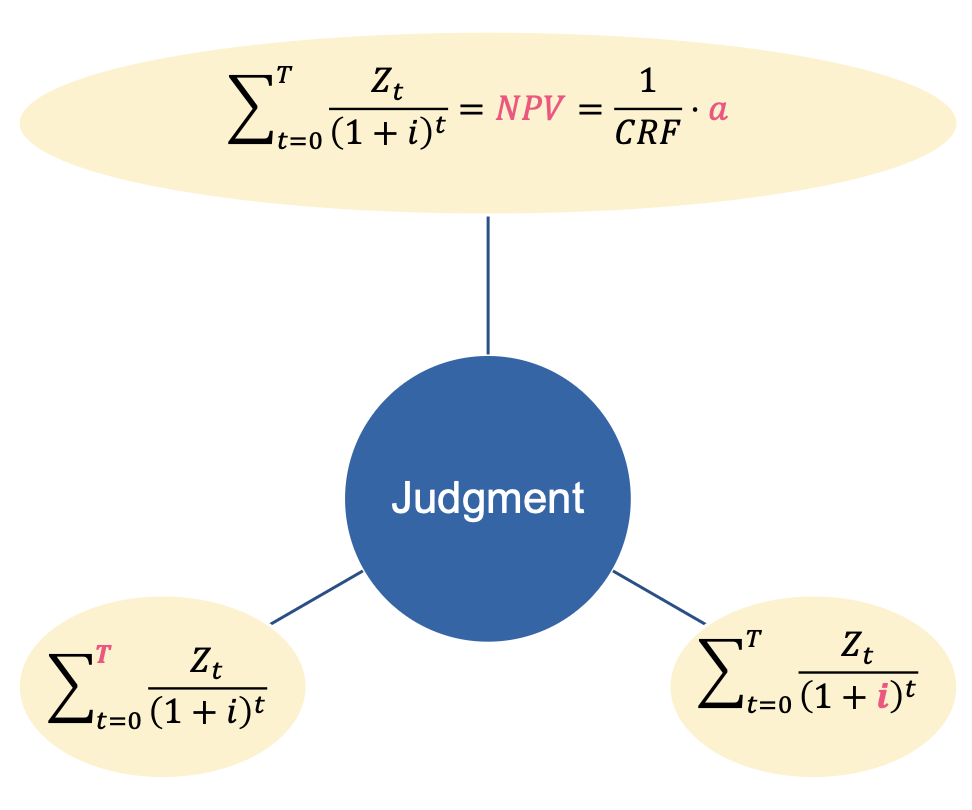
\includegraphics[width=0.3\textwidth]{images/investment-decision.png}
    \caption{The three judgement dimensions influencing investment decisions by T. Herrmann}
    \label{fig:investment_decision}
\end{figure}

\textbf{Net Present Value (NPV)} \\
The NPV sums the present value of all cash flows over the asset lifetime. If positive, it is profitable.

\begin{equation}
\label{eq:npv_equation}
\text{NPV} = Z_0 + \sum_{t=0}^{T} \frac{Z_t}{(1 + i)^t}
\end{equation}

\noindent
where $Z_0$ represents the initial investment cost at $t=0$ and $Z_t$ are the cash flows (costs or revenues) 
in period $t$.

By repeating the NPV calculation for each scenario, we can compare the financial viability of different 
investment options. The scenario with the highest positive NPV is the most profitable one.

\textbf{Annuity} \\
An other dynamyic decison making metric is the \emph{annuity} which permits to assess decison making on assets
with different lifetimes. It denotes an equivalent constant monetary input over the period under consideration.

Is calculated calculated from the NPV by multiplying it by the annuity factor (Capital Recovery Factor, CRF) :

\begin{equation}
\label{eq:annuity_equation}
a = NPV \cdot \frac{i (1 + i)^T}{(1 + i)^T - 1} = NPV \cdot CRF
\end{equation}

\textbf{Sensitivity Analysis} \\
While sensitivity analyses typically focus on varying discount rates, we instead analyze load variations 
($\pm20\%$) since interest rates were already discussed in Section~\ref{sec:data_preprocessing}. This helps 
assess both investment robustness, under demand uncertainty and identify potential risk of network constraints 
requiring additional capacity.


\subsubsection{Automatic AI-Based Reporting}
\label{sec:ai_reporting}

% A final, optional feature involves generating textual summaries via \textbf{OpenAI API}~\cite{openai_api_docs}
% calls in \texttt{scenario\_critic.py}. After each scenario's DCOPF run and financial calculations:
% \begin{itemize}
%   \item \textbf{Scenario Data Collection}: The script compiles key metrics (annual cost, NPV, etc.) and 
%   sends them to an LLM endpoint.
%   \item \textbf{Markdown Report Augmentation}: The LLM returns a short descriptive or analytic paragraph 
%   (e.g., identifying dominant cost drivers or storage benefits), which is appended to \texttt{.md} reports.
% \end{itemize}

% Moreover, the script automatically generates individual Markdown reports for each scenario including related 
% metrics and creates a global summary report that synthesizes insights across all scenarios, enabling quick 
% comparison of key findings and trade-offs.

% \paragraph{AI-Based Reporting and Automatic Reports: }
This module, \texttt{scenario\_critic.py}, integrates scenario data (annual costs, generator dispatch, net
present values, etc.) with an AI-based module to automatically produce Markdown reports for each scenario. 
Concretely, it performs:

\begin{enumerate}
    \item \textbf{API Integration} \\
    A class (\lstinline|ScenarioCritic|) initializes an OpenAI client using an API key~\cite{openai_api_docs}. We 
    define a "context prompt" describing the energy system mix (nuclear, gas, wind, etc.), relevant 
    cost metrics, and storage assets. 

    \item \textbf{Generating a Critical Analysis} \\
    The script collects scenario outputs (e.g. annual\_cost, generation by asset, etc.) into 
    a short "user" prompt. It requests an AI-generated critique. We chose to focus on the economic efficiency, 
    strengths/weaknesses, and possible improvements. This feedback is concise (up to 200 words) and helps users 
    quickly assess each scenario.

    \item \textbf{Automatic Markdown Reports.} \\
    Using both values from the optimization/investment metrics module and the AI critique, 
    the script compiles a scenario-specific \texttt{.md} file (e.g., 
    \lstinline|scenario_1_analysis.md|). 
    An example of the reports can be found in the Appendix.
    The final report includes:
    \begin{itemize}
        \item \emph{Key Financial Metrics}: Initial investment, annual cost, various NPVs.
        \item \emph{Generation Statistics}: Generation costs by asset, capacity factors, seasonal trends.
        \item \emph{AI Critical Analysis}: The generated text is appended to the report’s conclusion, 
        providing a quick executive-level summary.
        \item \emph{Plots and Figures}: If configured, the script references or embeds seasonal 
        generation comparisons and annual summaries.
    \end{itemize}
\end{enumerate}

% \begin{figure}[H]
%   \centering
%   \begin{tikzpicture}[%
%       every node/.style={draw, rectangle, rounded corners=2pt, font=\small, align=center},
%       node distance=4mm,
%       on grid,
%   ]
  
%   % Title box
%   \node[fill=gray!20, text width=7cm, minimum height=0.8cm] (title) {%
%       \textbf{Scenario Analysis Report: scenario\_X}\\
%       \small{Generated on: YYYY-MM-DD HH:MM}
%   };
  
%   % Plots row
%   \node[fill=blue!10, below=of title, text width=3.5cm, minimum height=2cm] (plot1) {Plot 1\\(Season Comparison)};
%   \node[fill=blue!10, right=3mm of plot1, text width=3.5cm, minimum height=2cm] (plot2) {Plot 2\\(Annual Summary)};
%   \node[fill=blue!10, below=3mm of plot2, text width=3.5cm, minimum height=2cm] (plot3) {Plot 3\\(Scenario Comparison)};
%   \node[draw=none, below=1mm of plot1] (dummy) {};
  
%   % Key metrics box
%   \node[fill=green!20, below=3mm of dummy, text width=7.2cm, minimum height=2cm] (metrics) {%
%       \textbf{Key Metrics}\\
%       \footnotesize \begin{tabular}{ll}
%       Initial Investment: & €X,XXX,XXX \\
%       Annual Cost: & €X,XXX,XXX \\
%       NPV (10\,y): & €X,XXX,XXX
%       \end{tabular}
%   };
  
%   % Generation stats
%   \node[fill=orange!10, below=3mm of metrics, text width=7.2cm, minimum height=2.2cm] (genstats) {%
%       \textbf{Generation / Costs / Capacity Factors}\\
%       \footnotesize \begin{verbatim}
% nuclear: 12345 MWh
% gas: 6789 MWh
% solar: 1357 MWh
%       \end{verbatim}
%   };
  
%   % AI summary box
%   \node[fill=red!10, below=3mm of genstats, text width=7.2cm, minimum height=1.8cm] (ai) {%
%       \textbf{AI Critical Analysis}\\
%       \footnotesize
%       "This scenario effectively balances X and Y,
%       but shows some reliance on gas. We recommend
%       additional storage to mitigate..."
%   };
  
%   % Title at top
%   \draw (title.south) -- (plot1.north);
%   \end{tikzpicture}
%   \caption{A schematic mockup of the generated scenario report layout.}
%   \label{fig:sketch-report}
% \end{figure}

\textbf{Cost Analysis} \\
It is important to note that the OpenAI API has a cost -- $0.00015$ USD per token. As seen in the Figure below on 
the 29th of January 2025, for our 12 scenarios plus 1 global (summary) report, it costed us \$0.0035 USD 
($\pm$ \$0.00027 per scenario). While negligible compared to the investment decisions analyzed sums, this is not 
a free feature. Other open-source LLMs usage could be evaluated.

\begin{figure}[H]
    \centering
    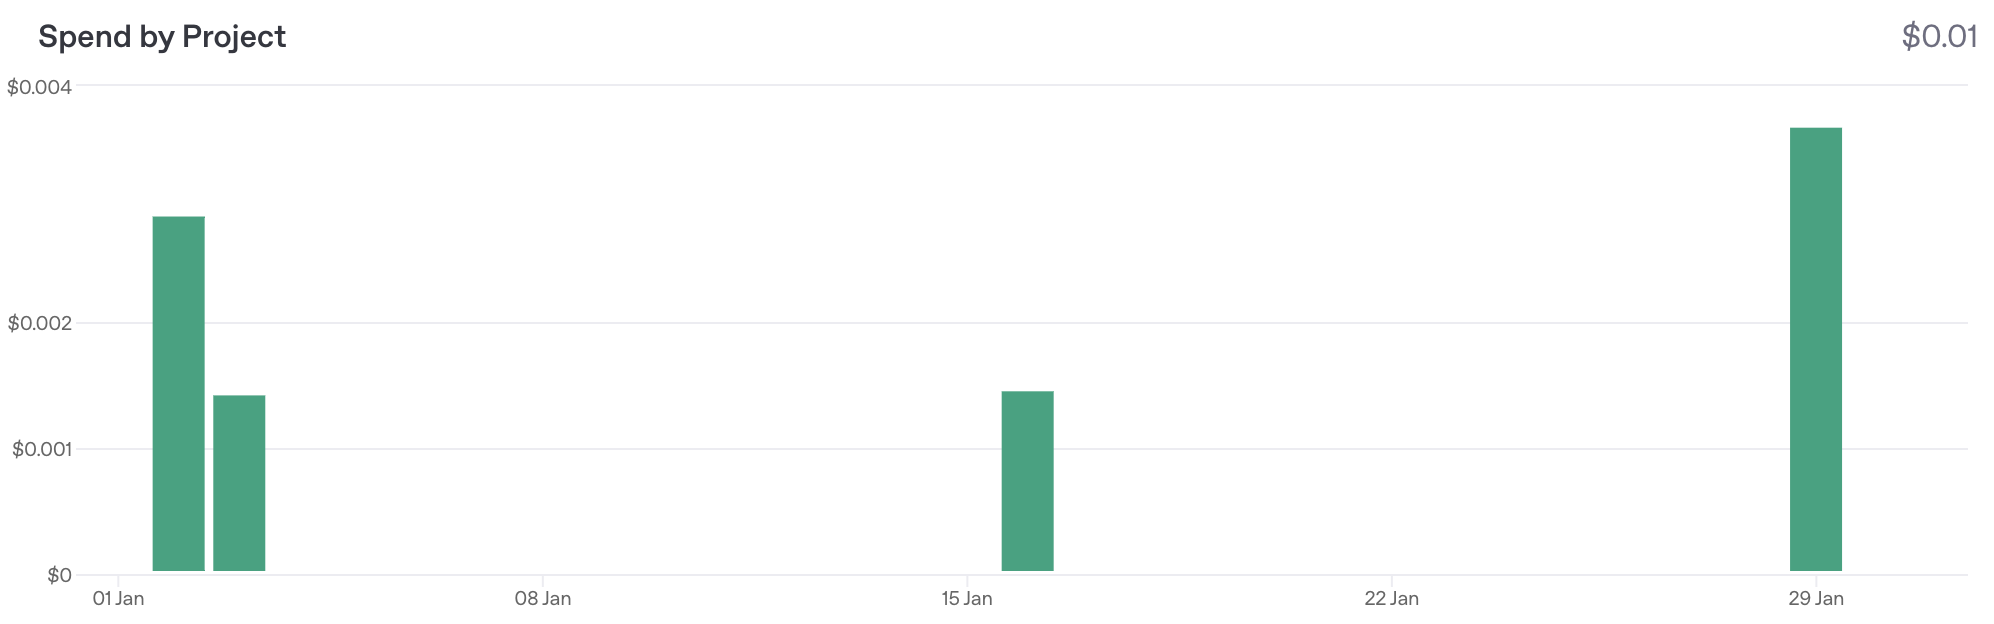
\includegraphics[width=0.75\textwidth]{images/api-cost.png}
    \caption{January 2025 project cost chart of OpenAI API Usage (Report Generation only)}
    \label{fig:api-cost}
\end{figure}

The AI analysis feature was implemented as an optional component that can be enabled or disabled according to user 
preference prior to running the optimization process. Hence guaranteeing that the platform can be used by users 
completely free of costs.


%---------------------------------------------------------------------------------------
\subsection{Technical Implementation}
\label{sec:technical_implementation}

This section covers the practical aspects of using Python and related libraries for solving the 
DCOPF and generating scenario results. It also addresses performance considerations.

\subsubsection{Programming Language \& Libraries}
\label{sec:programming_libraries}

All scripts are written in Python 3.10, leveraging the following key libraries:
\begin{itemize}
  \item \texttt{pulp} for linear programming and interfacing with \texttt{CBC} \cite{forrest2018cbc}. The verssion used is 2.9.0.
  \item \texttt{pandas}, \texttt{numpy}, and \texttt{matplotlib}/\texttt{seaborn} for data manipulation and
  visualization.
  \item \texttt{networkx} for optional graph-based analyses (e.g., if we extend to network exploration).
  \item \texttt{openai} for LLM access and generation of reports.
\end{itemize}


It was decided to use Poetry for dependency management and packaging, ensuring consistent versions across 
different environments. A detail .toml listing all dependencies is available if needed. Poetry facilitates 
the containerization of the platform.

While parts of the project are designed for containerization, certain components like the OpenAI API key require 
secure handling of personal credentials. Currently, the project runs locally without containerization, 
though its architecture was developed with it in mind.

\subsubsection{Performance}
\label{sec:performance_scalability}

While the solver has successfully handled a handful of scenarios (e.g., 20--40), it has yet to be benchmarked 
against large-scale or more complex networks. As order of magnitude, we computed different scenarios 
including sensitivity analysis and scenario plot generation enabled. No AI report generation was enabled.
We yield a linear correlation :

\begin{figure}[h]
    \centering
    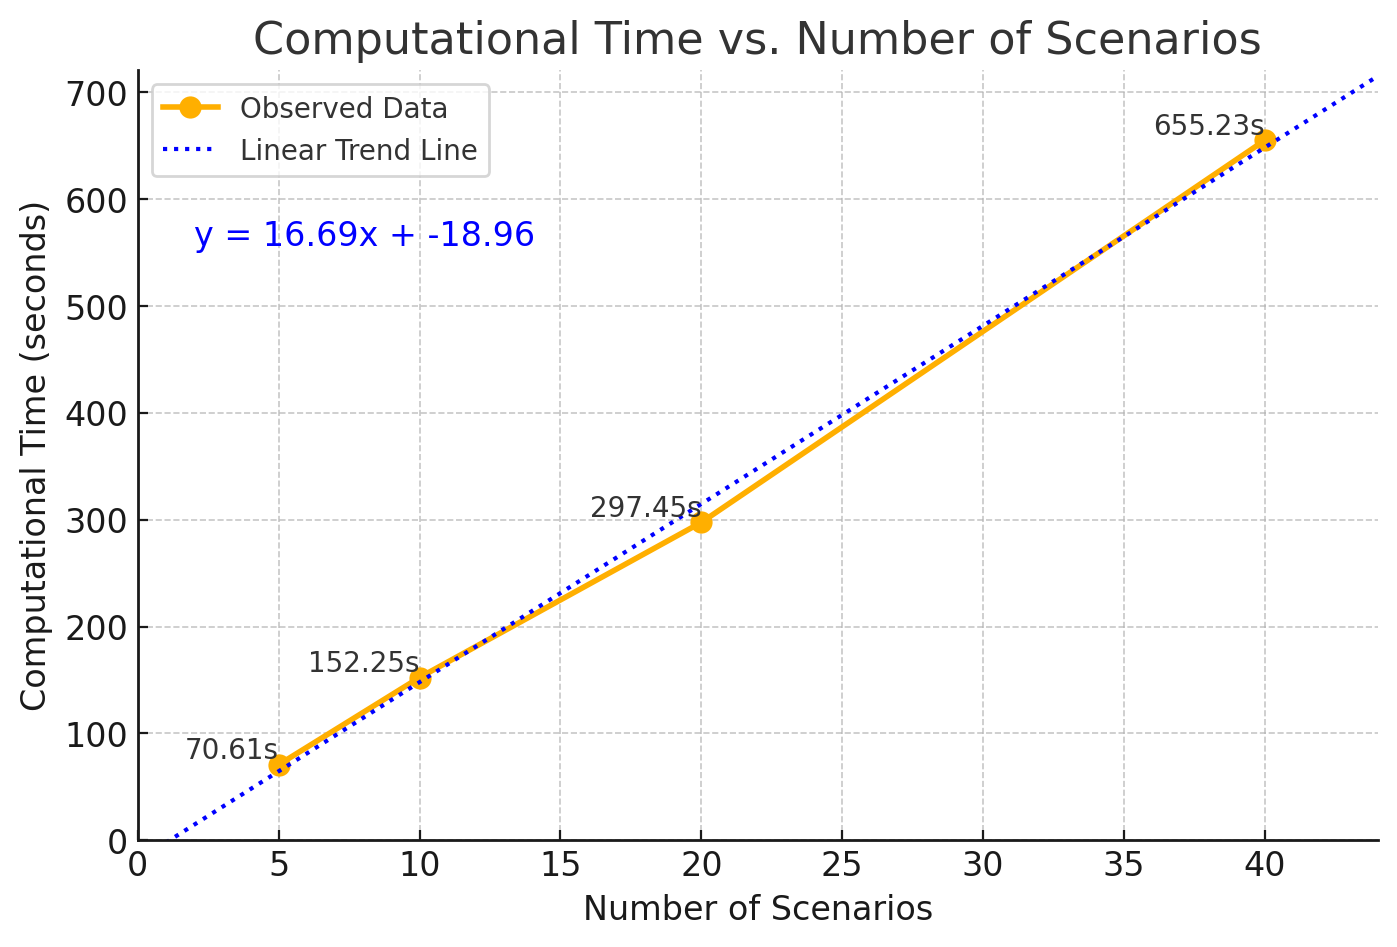
\includegraphics[width=0.5\textwidth]{images/time-comput.png}
    \caption{Computation time vs number of scenarios (correlation for limited number of scenarios only)}
    \label{fig:computation-time}
\end{figure}

As this was my first major programming project beyond small scripts, I prioritized a flexible, 
readable codebase over computational efficiency. Nonetheless, handling hourly time-series data for an 
entire year inherently creates a large number of constraints (over 8,700). Real-world systems even adopt 
finer temporal resolutions (e.g., 15-minute intervals). 

To keep run times feasible, we selected representative weeks per season—an approach that cuts computing by 
roughly 17x. (With 52 weeks in a year reduced to just 3 representative weeks -- 52/3 = 17).

% \subsubsection{Validation Checks (Optional)}
% \label{sec:validation_checks}

% Internally, the DCOPF solver in \texttt{dcopf.py} outputs:
% \begin{itemize}
%   \item \textbf{Solver Status}: Confirms if the final status is \texttt{Optimal} (code = 1). Otherwise, 
%   the script prints diagnostic messages.
%   \item \textbf{Power Balance Consistency}: Each bus has an equality constraint ensuring generation plus 
%   inflow equals demand plus outflow.
%   \item \textbf{Line Flow Limits}: Each line’s power flow is constrained by \texttt{rateA}, preventing 
%   unrealistic transfers.
% \end{itemize}
% When executed, the script logs each step, making it relatively straightforward to trace and debug any 
% infeasibilities or unexpected cost spikes. Although no separate “checksum” routine is implemented at 
% present, these logs provide a practical first-level validation of each scenario run.

% \bigskip
% \noindent
% \textbf{In summary, the technical choices---a Python stack, Poetry-driven package management, and a DCOPF 
% solver in \texttt{pulp}---offer a clean, reproducible workflow.} While current tests focus on a limited 
% number of scenarios and relatively small networks, the methodology can be scaled with additional 
% optimization or ML-based strategies for high-volume scenario analyses.